\documentclass[11pt,a4paper]{article}

\usepackage[T1]{fontenc}
\usepackage[utf8]{inputenc}
\usepackage{mathpazo}
\usepackage[margin=2.3cm]{geometry}
\usepackage{microtype}
\usepackage{amsmath,mathtools}
\usepackage{siunitx}
\usepackage{booktabs,tabularx,array,longtable}
\usepackage{graphicx}
\usepackage[font=small,labelfont=bf]{caption}
\usepackage[shortlabels]{enumitem}
\usepackage{xcolor}
\usepackage{fancyhdr}
\usepackage{titlesec}
\usepackage[colorlinks=true,linkcolor=accent,urlcolor=accent,citecolor=accent]{hyperref}

\definecolor{accent}{HTML}{0F6E56}
\titleformat{\section}{\large\bfseries\color{accent}}{\thesection\quad|}{0.6em}{\MakeUppercase}
\titleformat{\subsection}{\normalsize\bfseries}{\thesubsection\quad|}{0.6em}{}
\titlespacing*{\section}{0pt}{14pt}{6pt}
\titlespacing*{\subsection}{0pt}{10pt}{4pt}

\pagestyle{fancy}
\fancyhf{}
\fancyfoot[L]{\small\color{gray}A virtual perfusion bioreactor and digital shadow of CAR T cell expansion}
\fancyfoot[R]{\small\thepage}
\renewcommand{\headrulewidth}{0pt}

\sisetup{per-mode=symbol}
\newcommand{\code}[1]{\texttt{#1}}
\newcommand{\dd}{\mathrm{d}}
\newcommand{\kla}{k_La}
\newcommand{\tlag}{t_{\mathrm{lag}}}
\newcommand{\tsed}{t_{\mathrm{sed}}}
\newcommand{\mumax}{\mu_{\max}}
\newcommand{\Ssp}{[S_{\mathrm{sp}}]}
\newcommand{\cS}{[S(t)]}
\newcommand{\cP}{[P(t)]}
\newcommand{\cX}{[X(t)]}
\setlength{\parskip}{4pt}
\setlength{\parindent}{0pt}
\setlist{nosep, leftmargin=*}
\renewcommand{\arraystretch}{1.15}

\title{\color{accent}\textbf{A virtual perfusion bioreactor and digital shadow of\\ CAR T cell expansion}\\[4pt]
\large Technical documentation of the \code{closed-loop-cell-therapy} repository}
\author{Luxi Yu}
\date{Version 0.2.0}

\begin{document}
\maketitle
\thispagestyle{fancy}

\begin{abstract}
\noindent To manufacture chimeric antigen receptor (CAR) T cells of the desired quantity and
quality, the cells must be expanded ex vivo for an optimal duration, which in turn requires
knowledge of the cell concentration during the expansion period. Egan et al.\ (2025) developed a
digital shadow of CAR T cell expansion that provides a soft sensor of cell concentration in real
time: a mechanistic model of cell growth within a proportional-integral-derivative (PID) controlled
perfusion bioreactor, fitted to online data of the perfusion rate and the glucose and lactate
concentrations. The present work re-implements that digital shadow and, because the original
datasets are proprietary, embeds it in a virtual bioreactor that generates online and off-line data
for six bioreactor runs of the Aglaris FACER from the published model parameters. The virtual
bioreactor adds sensor noise, bubble artefacts, the published low-pass filter, PID feedback on the
filtered glucose signal and a mechanical fault. Digital shadow training recovers the yield
parameters to within 5\%. Real-time testing shows that with 2.5~days of online data the final cell
concentration is predicted with a mean relative error of 8\% (maximum 23\%), compared with 13\%
reported by Egan et al. As in the original study, the confidence bands are too narrow, because the
uncertainty in the fixed parameters $Y_{xs}$ and $\tlag$ is not propagated.
\end{abstract}

\textbf{Keywords:} cell growth, digital shadow, mathematical model, PID control, predictive model,
process analytical technology, soft sensor

\tableofcontents

% =====================================================================
\section{Introduction}

Prolonged ex vivo expansion has been associated with progressive differentiation of CAR T cells
that can result in less effective treatment, whereas activated CAR T cells must be administered at a
sufficiently high dose to be effective \cite{egan2025}. Both the quality and the quantity of CAR T
cells are therefore critical quality attributes (CQAs), and the optimal harvest time is patient
specific. Hard sensors such as dielectric spectroscopy are less suited to bioreactors in which the
cells grow whilst sedimented on a membrane, and resuspending the cells for off-line analysis risks
breaching the sterility barrier and can disturb continued cell growth.

Egan et al.\ \cite{egan2025} addressed this with a digital shadow, defined as a virtual
representation with a one-way transfer of data from the physical to the virtual component (in
contrast to a digital twin, which transfers data in both directions and can adaptively control the
physical system). The digital shadow provides nowcasts and short-term forecasts of the cell
concentration from the hard sensors already used to monitor and control the process.

This document describes a re-implementation of that work with two purposes: (i) to reproduce the
digital shadow and its training and testing procedures, and (ii) to provide a virtual bioreactor in
which the digital shadow, and later extensions such as ensemble-based estimation and supervisory
decision support, can be developed and tested without access to the proprietary datasets.

% =====================================================================
\section{Materials and methods}

\subsection{Mathematical}

\textbf{Batch-perfusion process.} Cells with concentration $\cX$ are seeded at time $t_I$ and retained
in the bioreactor via sedimentation. Perfusion does not begin immediately at $t_I$ but at $\tsed$,
after which fresh media with glucose concentration $[S_I]$ is perfused into the bioreactor at a
rate $D(t)$, and spent media with glucose and lactate concentrations $\cS$ and $\cP$ is perfused out
at the same rate, maintaining a constant volume $V$. The perfusion rate is
\begin{equation}
  D(t) = Q(t)/V, \label{eq:D}
\end{equation}
where $Q(t)$ is the volumetric flow rate; $D(t)=\SI{1}{\per\day}$ corresponds to one vessel volume
per day (VVD). The contents of the bioreactor are modelled as homogeneous; the model is of the
unstructured and unsegregated type and is formulated via nonlinear ordinary differential equations
(ODEs). Following Egan et al., the following assumptions are made: the flow rate is sufficiently
small that only a negligible number of cells are removed in the effluent; glucose and lactate
concentrations have a negligible inhibitory effect on cell growth; the dominant inhibitory effect is
due to the cells competing with each other to grow in a space-limited environment; cell death and
maintenance are negligible; and the growth yield factors are constant.

\textbf{Cell growth model.} The cell concentration and specific growth rate are given by a lag period
$\tlag - t_I$ followed by a special case of the Richards growth model \cite{richards1959}, applicable in
the early stages of cell growth when $\cX \ll [K]$:
\begin{align}
  \cX &= \frac{[X_I]}{\bigl(1 - H(t-\tlag)\,\mumax\,\nu\,(t-\tlag)\bigr)^{1/\nu}} \quad \text{for } t\ge t_I \text{ and } \nu<0, \label{eq:X}\\
  \mu(t) &= \frac{H(t-\tlag)\,\mumax}{1 - H(t-\tlag)\,\mumax\,\nu\,(t-\tlag)} \quad \text{for } t\ge t_I \text{ and } \nu<0, \label{eq:mu}
\end{align}
where $[X_I]$ is the initial cell concentration, $\mumax$ is the maximum specific growth rate at
$\tlag$, $\nu$ determines the decrease of the specific growth rate over time, and $H$ denotes the
Heaviside step function (eqs~10, 11 and S60, S61 of \cite{egan2025}). Substituting $\nu=-1$ gives
approximately linear cell growth and $\nu=-1/2$ approximately quadratic growth; increasingly small
values of $\nu$ recover the limiting case of exponential growth (Figure~\ref{fig:growth}).

\begin{figure}[h]
\centering
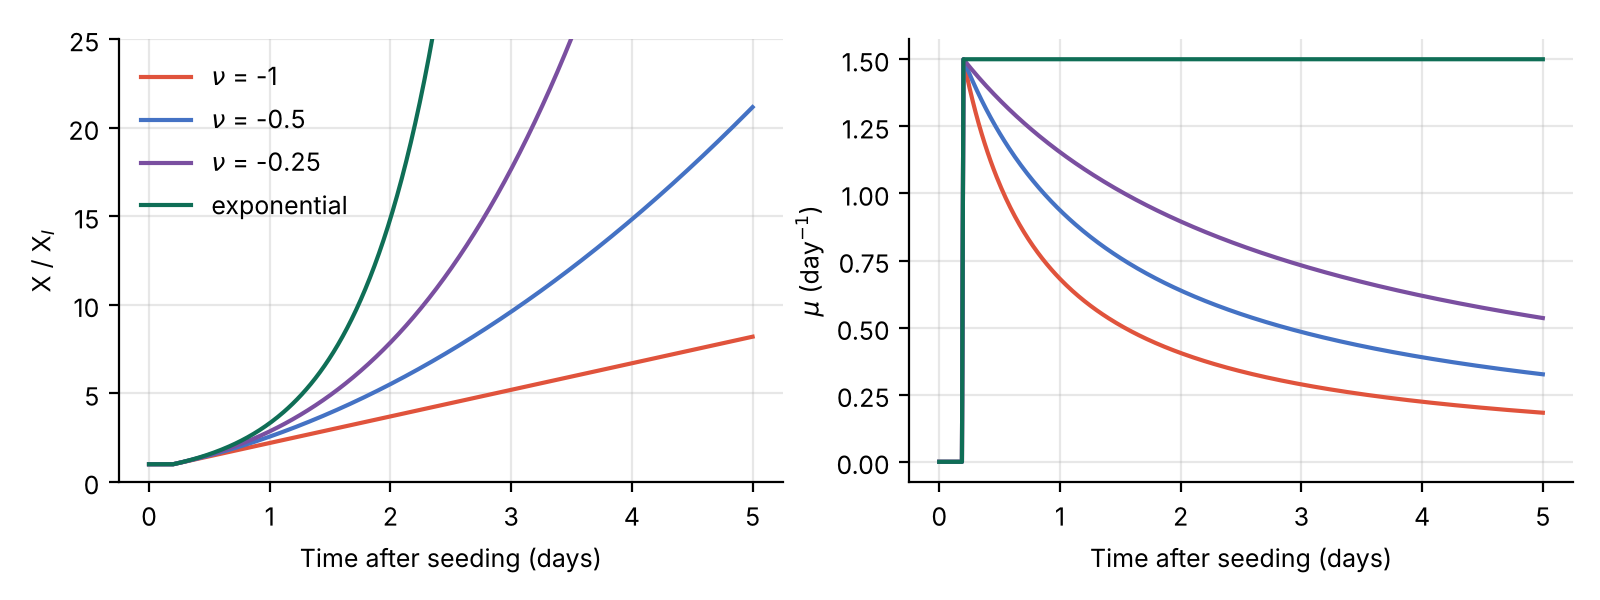
\includegraphics[width=0.88\textwidth]{figures/growth_family.png}
\caption{Cell concentration (left) and specific growth rate (right) given by
equations~\eqref{eq:X} and~\eqref{eq:mu} for $\mumax = \SI{1.5}{\per\day}$,
$\tlag - t_I = 0.2$~days and four values of $\nu$.}
\label{fig:growth}
\end{figure}

If the final cell concentration $[X_F]$ at time $t_F$ is known, $\mumax$ can be given as a
combination of the other parameters, and equation~\eqref{eq:X} can be rearranged to give the time
$t_T$ at which the cell concentration reaches a threshold concentration $[X_T]$:
\begin{equation}
  \mumax = \frac{1-([X_I]/[X_F])^{\nu}}{\nu\,(t_F-\tlag)}, \qquad
  t_T = \tlag + \frac{1-([X_I]/[X_T])^{\nu}}{\mumax\,\nu} \quad \text{for } \nu<0. \label{eq:closed}
\end{equation}

\textbf{Glucose, lactate and PI controlled perfusion rate.} The glucose and lactate concentrations
and the perfusion rate are modelled as
\begin{align}
  \frac{\dd[S]}{\dd t} &= H(t-\tsed)\,D(t)\,([S_I] - \cS) - \frac{\mu(t)\cX}{Y_{xs}} \quad \text{for } t\ge t_I, \label{eq:S}\\
  \frac{\dd[P]}{\dd t} &= Y_{px}\,\mu(t)\cX - H(t-\tsed)\,D(t)\,\cP \quad \text{for } t\ge t_I, \label{eq:P}\\
  \frac{\dd D}{\dd t} &= H(t-\tsed)\Bigl(K_p\,\frac{\dd(\Ssp - \cS)}{\dd t} + K_i\,(\Ssp - \cS)\Bigr) \quad \text{for } t\ge t_I, \label{eq:PI}
\end{align}
where $Y_{xs}$ and $Y_{px}$ denote the yield of cells from glucose and the yield of lactate from
cells, respectively, $\Ssp$ is the glucose concentration set-point, and $K_p$ and $K_i$ are the
proportional and integral gains (eqs~2--4 of \cite{egan2025}). Equation~\eqref{eq:PI} models the PID
controller as a proportional-integral (PI) controller, a good approximation since the derivative
gain $K_d$ is 3--4 orders of magnitude smaller than $K_p$ and $K_i$. The yield of lactate from
glucose is
\begin{equation}
  Y_{ps} = Y_{px}\,Y_{xs}. \label{eq:Yps}
\end{equation}
Assuming that, for $t\ge t_{sp}$, the glucose concentration remains approximately at its set-point,
$\dd[S]/\dd t\approx 0$, and the lactate concentration tends to the steady state
\begin{equation}
  [P_{ss}] = Y_{ps}\,([S_I] - \Ssp), \label{eq:Pss}
\end{equation}
which is the yield of lactate from glucose multiplied by the difference between the glucose
concentration in the fresh media and the glucose concentration set-point (eq.~18 of \cite{egan2025}).

\textbf{Dissolved oxygen.} For the extended model, the normalised dissolved oxygen (DO)
$C'(t)=[C(t)]/[C^*]$ is modelled as
\begin{equation}
  \frac{\dd C'}{\dd t} = \bigl(H(t-\tsed)\,D(t) + \kla\bigr)\bigl(1 - C'(t)\bigr) - \frac{\mu(t)\cX}{Y'_{xc}}
  \quad \text{for } t\ge t_I, \label{eq:DO}
\end{equation}
where $\kla$ is the volumetric mass transfer coefficient and $Y'_{xc}=Y_{xc}[C^*]$ is the scaled yield
of cells from DO (eqs~8, 9 of \cite{egan2025}).

\textbf{Discrete solution.} The perfusion rate, glucose concentration and lactate concentration have a
lower bound of zero. Following Egan et al., equations~\eqref{eq:S}--\eqref{eq:PI} and~\eqref{eq:DO}
are approximated by forward finite difference equations and solved via the forward Euler method
with a step size of \SI{10}{\second}:
\begin{align}
  [S(t_{k+1})] &= \max\Bigl(0,\ [S(t_k)] + \Delta t\Bigl(D(t_k)([S_I]-[S(t_k)]) - \frac{\mu(t_k)[X(t_k)]}{Y_{xs}}\Bigr)\Bigr), \label{eq:S22}\\
  D(t_{k+1}) &= \max\Bigl(D_{\min},\ D(t_k) - K_p\bigl([S(t_{k+1})]-[S(t_k)]\bigr) + \Delta t\,K_i\bigl(\Ssp - [S(t_k)]\bigr)\Bigr), \label{eq:S23}\\
  [P(t_{k+1})] &= \max\Bigl(0,\ [P(t_k)] + \Delta t\bigl(Y_{px}\,\mu(t_k)[X(t_k)] - D(t_k)[P(t_k)]\bigr)\Bigr), \label{eq:S24}
\end{align}
with $t_0=\tsed$ and $D(t_0)=D_{\min}$ (eqs~S22--S24). $\cX$ and $\mu(t)$ are evaluated analytically
from equations~\eqref{eq:X} and~\eqref{eq:mu}. The implementation is \code{process/facer.py}.

\subsection{Virtual bioreactor}

\textbf{Culture system.} The virtual bioreactor represents the large chamber of the Aglaris FACER, a
completely closed and automated cell production system with a single-use cartridge of two culture
chambers (volumes of \SI{13.4}{\milli\litre} and \SI{134}{\milli\litre}, surface areas of
\SI{10}{\centi\metre\squared} and \SI{100}{\centi\metre\squared}). Within the culture chambers,
cells are cultivated under static conditions on a gas-permeable membrane that separates the
controlled media zone from the controlled gas zone.

\textbf{Process dynamics.} The virtual bioreactor (\code{sim/runner.py}) evolves
equations~\eqref{eq:X}, \eqref{eq:mu}, \eqref{eq:S}, \eqref{eq:P} and~\eqref{eq:DO} with the step
size of \SI{10}{\second} and the parameter values of a given bioreactor run. Unlike the digital
shadow, the perfusion rate is set by a PID controller (\code{control/perfusion.py}) acting on the
filtered online glucose signal, in the velocity form
\begin{equation}
\begin{gathered}
  D(t_{k+1}) = \max\Bigl(D_{\min},\ D(t_k) + K_p(e_{k+1}-e_k) + K_i\,\Delta t\,e_k + K_d\,\frac{e_{k+1}-2e_k+e_{k-1}}{\Delta t}\Bigr),\\
  e_k = \Ssp - [\tilde S(t_k)],
\end{gathered}
  \label{eq:pid}
\end{equation}
where $[\tilde S]$ denotes the filtered glucose measurement; with $K_d=0$ and $[\tilde S]=[S]$ this
reduces to equation~\eqref{eq:S23}.

\textbf{Online data.} Glucose and lactate concentrations are measured every \SI{10}{\second} via
enzymatic sensors, with additive Gaussian noise (standard deviation \SI{0.08}{\milli\mole\per\litre}).
Bubbles generated during the expansion process interfere with the online sensors, leading to
artificial drops in the glucose and lactate concentration readings followed by rises once the bubbles
have moved away. These are modelled as a Poisson process (3 per day) in which the readings fall to a
fraction of 0.3--0.8 of the true concentration for 20--\SI{300}{\second}. To prevent these
fluctuations impacting the perfusion rate, the raw glucose and lactate data are filtered before being
passed to the PID controller by a lowpass Butterworth filter of order 2 with a cut-off frequency of
\SI{0.001}{\hertz}, applied causally to the \SI{10}{\second} readings. Not all bubble artefacts are
filtered out, which results in downward spikes of the glucose (and lactate) concentration followed
by upward spikes in the perfusion rate (Figure~\ref{fig:bubble}). Normalised DO is recorded with
additive noise (standard deviation 0.01). The noise levels and bubble statistics are assumed values;
the filter specification is that of Egan et al.

\textbf{Off-line data.} Accurately measuring the cell concentration requires the cells to be in
suspension, and resuspending the cells after they have sedimented can disturb their growth.
Off-line cell counts are therefore generated only at $t_I$ and $t_F$, with a coefficient of variation
of 5\%.

\textbf{Mechanical issue.} In run~3, a mechanical issue occurred 2.5~days following the start of
perfusion and lasted for approximately 0.5~days, during which perfusion stopped and no online data of
the glucose and lactate concentrations were recorded. This is reproduced by setting $D(t)=0$ and
withholding all online data over $[\tsed+2.5,\ \tsed+3.0]$ days.

\textbf{Bioreactor runs.} Table~\ref{tab:runs} lists the observed (input) and best-fit (output)
parameters of the six runs, taken from Tables~1, 2 and~S4 of \cite{egan2025}
(\code{process/parameters.py}). All runs share $D_{\min}=\SI{0.067}{\per\day}$,
$K_p = \SI{0.215}{L\per(mmol.day)}$, $K_i = \SI{5.16}{L\per(mmol.day^2)}$,
$K_d = \SI{7.46e-5}{L\per mmol}$ and $V = \SI{134}{\milli\litre}$. In runs 1--5, cells were expanded in
TexMACS medium with IL-7 and IL-15 (media~A); in run~6, in Advanced TCM with IL-2 (media~B). Run~4
expanded patient CAR T cells; the others, donor T cells. Run~3 was the independent test dataset of
the original study and has no best-fit parameters; it is assigned the mean training values, with
$\mumax$ given by equation~\eqref{eq:closed} such that $[X(t_F)]=[X_F]$.

\begin{table}[h]
\centering\footnotesize
\setlength{\tabcolsep}{3.2pt}
\caption{Observed and best-fit parameters of the six bioreactor runs in the large chamber of the
Aglaris FACER \cite{egan2025}. Times in days from the start of the process; concentrations in
\si{\milli\mole\per\litre} and \num{e6}~cells/mL; $Y_{xs}$ in cells/pmol; $Y_{px}$ in pmol/cell;
$\kla$ in \si{\per\day}; $Y'_{xc}$ in \num{e6}~cells/mL. Italics: assigned values (run~3).}
\label{tab:runs}
\resizebox{\textwidth}{!}{%
\begin{tabular}{@{}l r r r r r r r r r r r r r r@{}}
\toprule
Run & $t_I$ & $\tsed$ & $t_F$ & $[S_I]$ & $\Ssp$ & $[X_I]$ & $[X_F]$ & $Y_{xs}$ & $Y_{px}$ & $\tlag-t_I$ & $\nu$ & $\mumax$ & $\kla$ & $Y'_{xc}$ \\
\midrule
1 & 0.11 & 0.34 & 5.05 & 25 & 20 & 1.49 & 19.0 & 0.231 & 7.93 & 0.160 & $-0.922$ & 2.14 & 3.00 & 3.68 \\
2 & 0.14 & 1.02 & 6.03 & 25 & 20 & 0.37 & 19.0 & 0.275 & 6.25 & 0.172 & $-0.477$ & 2.02 & 741 & 0.0220 \\
3 & 0.11 & 0.86 & 6.01 & 25 & 20 & 1.49 & 32.5 & \textit{0.259} & \textit{7.62} & \textit{0.092} & $\mathit{-0.537}$ & \textit{1.36} & \textit{3.00} & \textit{3.68} \\
4 & 2.09 & 2.84 & 7.00 & 25 & 20 & 0.62 & 10.9 & 0.272 & 9.09 & 0.128 & $-0.524$ & 1.39 & 1.73 & 6.27 \\
5 & 1.92 & 2.92 & 6.95 & 25 & 17 & 1.13 & 8.73 & 0.207 & 6.83 & 0.000 & $-0.000$ & 0.405 & 42.9 & 0.189 \\
6 & 0.08 & 0.83 & 4.85 & 26 & 21 & 1.49 & 18.2 & 0.311 & 7.99 & 0.000 & $-0.761$ & 1.58 & 20.2 & 0.893 \\
\bottomrule
\end{tabular}}
\end{table}

\subsection{Computational}

\textbf{Digital shadow.} The digital shadow (\code{shadow/fit.py}) is fitted simultaneously to the
perfusion rate, glucose concentration and lactate concentration data of each run; the three online
data sources are given equal weight and no scaling is applied. Equations~\eqref{eq:X},
\eqref{eq:mu} and~\eqref{eq:S22}--\eqref{eq:S24} are used in the fitting process. Fitting is
performed by nonlinear least-squares minimisation with the trust-region reflective method of SciPy,
which accommodates the parameter bounds $Y_{xs},Y_{px}>0$, $0\le\tlag-t_I<t_F-t_I$ and $\nu<0$ (Egan
et al.\ used the Levenberg--Marquardt method in the lmfit package). To reduce computation, the model
is evaluated on a \SI{60}{\second} grid and compared with the online data at the same time points.

\textbf{Digital shadow training.} For training purposes, data for both the initial and final cell
concentrations constrain the system via equation~\eqref{eq:closed}, so that $\mumax$ does not have to be
fitted directly; the fitted parameters are $Y_{xs}$, $Y_{px}$, $\tlag$ and $\nu$.

\textbf{Digital shadow testing.} In a real-time scenario, either the lag period or the maximum
specific growth rate must be known a priori for the model to be structurally identifiable
(Table~S1 of \cite{egan2025}); fixing the lag period alone leaves the model practically
unidentifiable. The lag period and the yield of cells from glucose are therefore fixed at their mean
training values ($\tlag-t_I=0.092$~days, $Y_{xs}=0.259$~cells/pmol), and $Y_{px}$, $\mumax$ and $\nu$
are fitted to the online data available at the time of model fitting. The real-time version is
fitted with 1.5 to 4~days of online data (in half-day time steps) from the start of perfusion; for
run~3, with 1.5 to 2.5~days, prior to the mechanical issue. The extended model including
equation~\eqref{eq:DO} is not used for fitting, since $\kla$ and $Y'_{xc}$ are not practically
identifiable from these data (Table~S4 of \cite{egan2025}).

\textbf{Confidence bands.} Confidence bands for $\cX$ and $\mu(t)$ are derived from the partial
derivatives with respect to $\mumax$ and $\nu$ (eqs~S67--S70) and the covariance matrix resulting
from the fitting process:
\begin{equation}
  \Delta f = \nabla f^{\mathsf T}\,\mathrm{cov}[\mumax,\nu]\,\nabla f, \qquad
  B = \hat f \pm \tau_{\alpha/2,n}\sqrt{\chi^2_n\,\Delta f}, \label{eq:band}
\end{equation}
where $f=\{\cX,\mu(t)\}$, $n$ is the number of degrees of freedom, $\chi^2_n$ is the reduced
chi-squared statistic and $\tau_{\alpha/2,n}$ is the upper $\alpha/2$ critical value of Student's $t$
distribution, with $\alpha=0.05$ (eqs~S71, S72).

% =====================================================================
\section{Results}

\subsection{Virtual bioreactor data}
Figure~\ref{fig:run1} shows the simulated online and off-line data of run~1 in the layout of Figure~3
of Egan et al. After the sedimentation period, the glucose concentration falls below its set-point,
the PI(D) controller increases the perfusion rate, and following an initial transient the glucose
concentration remains at \SI{20}{\milli\mole\per\litre} with an approximately constant perfusion rate,
consistent with the approximately linear cell growth for $\nu\approx-1$. The lactate concentration
approximately stabilises at a steady state shortly after the glucose concentration stabilises at its
set-point, in agreement with equation~\eqref{eq:Pss}. For all six runs, the simulated final cell
concentration equals the published $[X_F]$, the values of $\mumax$ and of the required expansion
period $t_T-t_I$ for $[X_T]=10^7$~cells/mL agree with Table~2 of \cite{egan2025} to within
0.015~day$^{-1}$ and 0.04~days, respectively, and the terminal lactate concentration is within 5\% of
$[P_{ss}]$.

\begin{figure}[p]
\centering
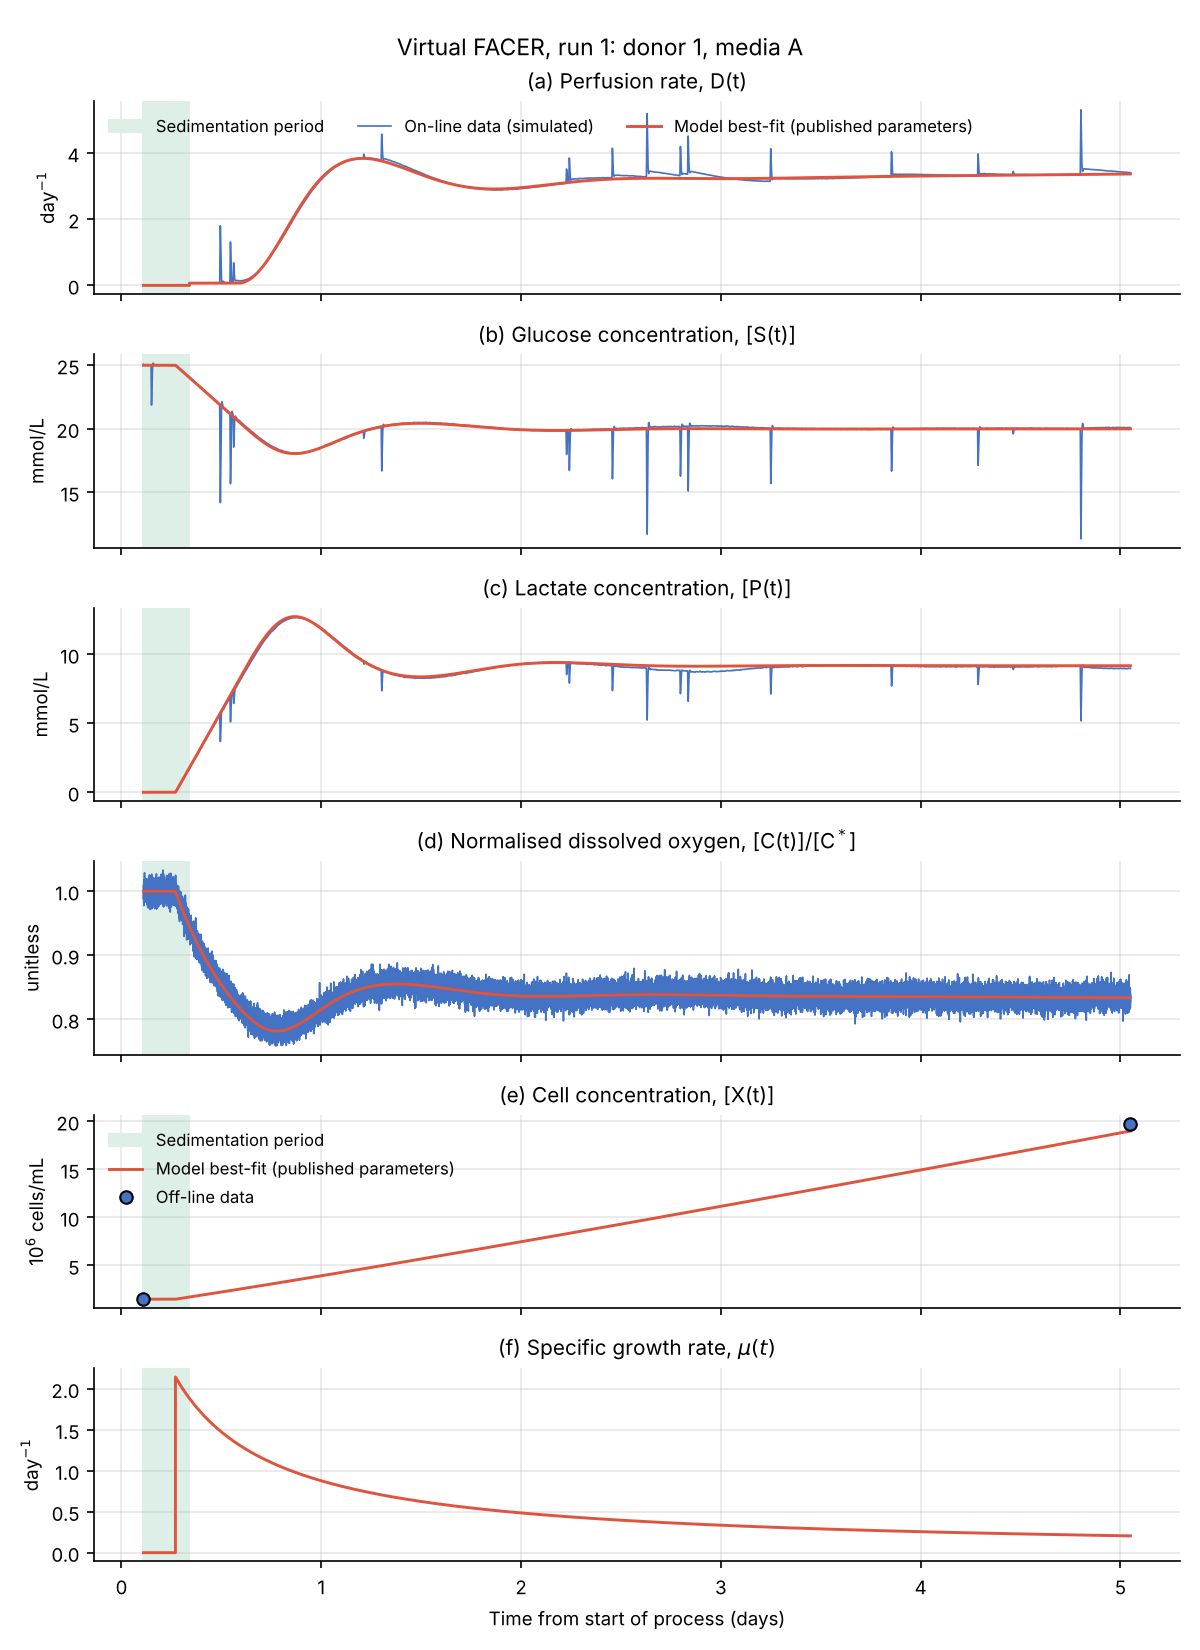
\includegraphics[width=0.8\textwidth]{figures/run1.png}
\caption{Key data from virtual run~1 in the large chamber of the FACER and model trajectories with
the published best-fit parameters (cf.\ Figure~3 of \cite{egan2025}).}
\label{fig:run1}
\end{figure}

\begin{figure}[h]
\centering
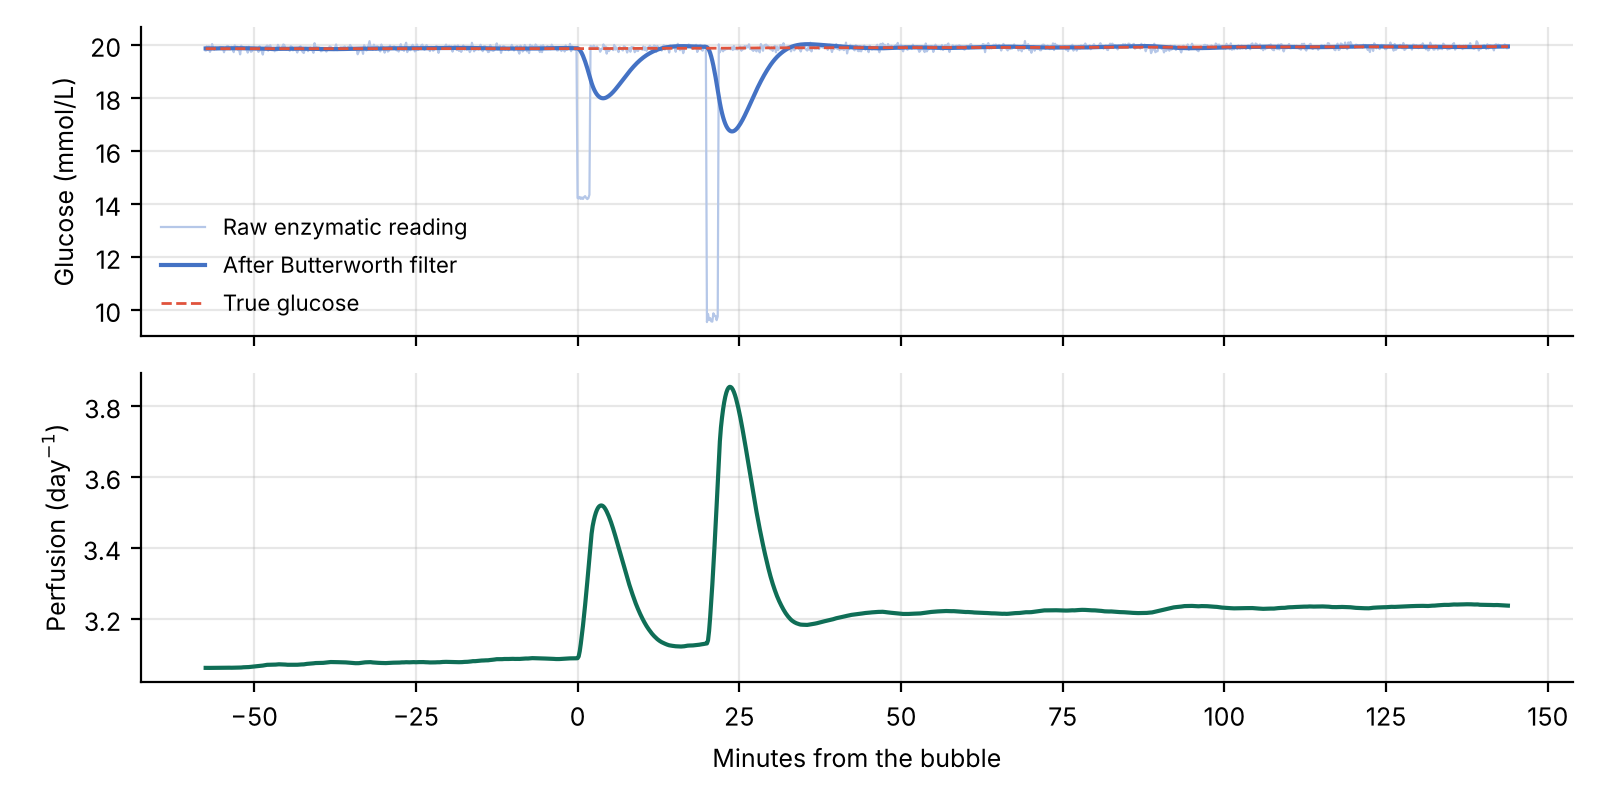
\includegraphics[width=0.85\textwidth]{figures/bubble_filter.png}
\caption{Two bubble artefacts in virtual run~1: raw and filtered glucose concentration (top) and the
resulting upward spikes in the perfusion rate (bottom).}
\label{fig:bubble}
\end{figure}

Figure~\ref{fig:run3} shows run~3. During the mechanical issue, perfusion stops, glucose is depleted
and lactate accumulates; on resumption, the controller drives the perfusion rate above the trajectory
of the undisturbed model before the glucose concentration returns to its set-point. Cell growth is
unaffected, in accordance with the model assumption of negligible substrate and product inhibition.

\begin{figure}[p]
\centering
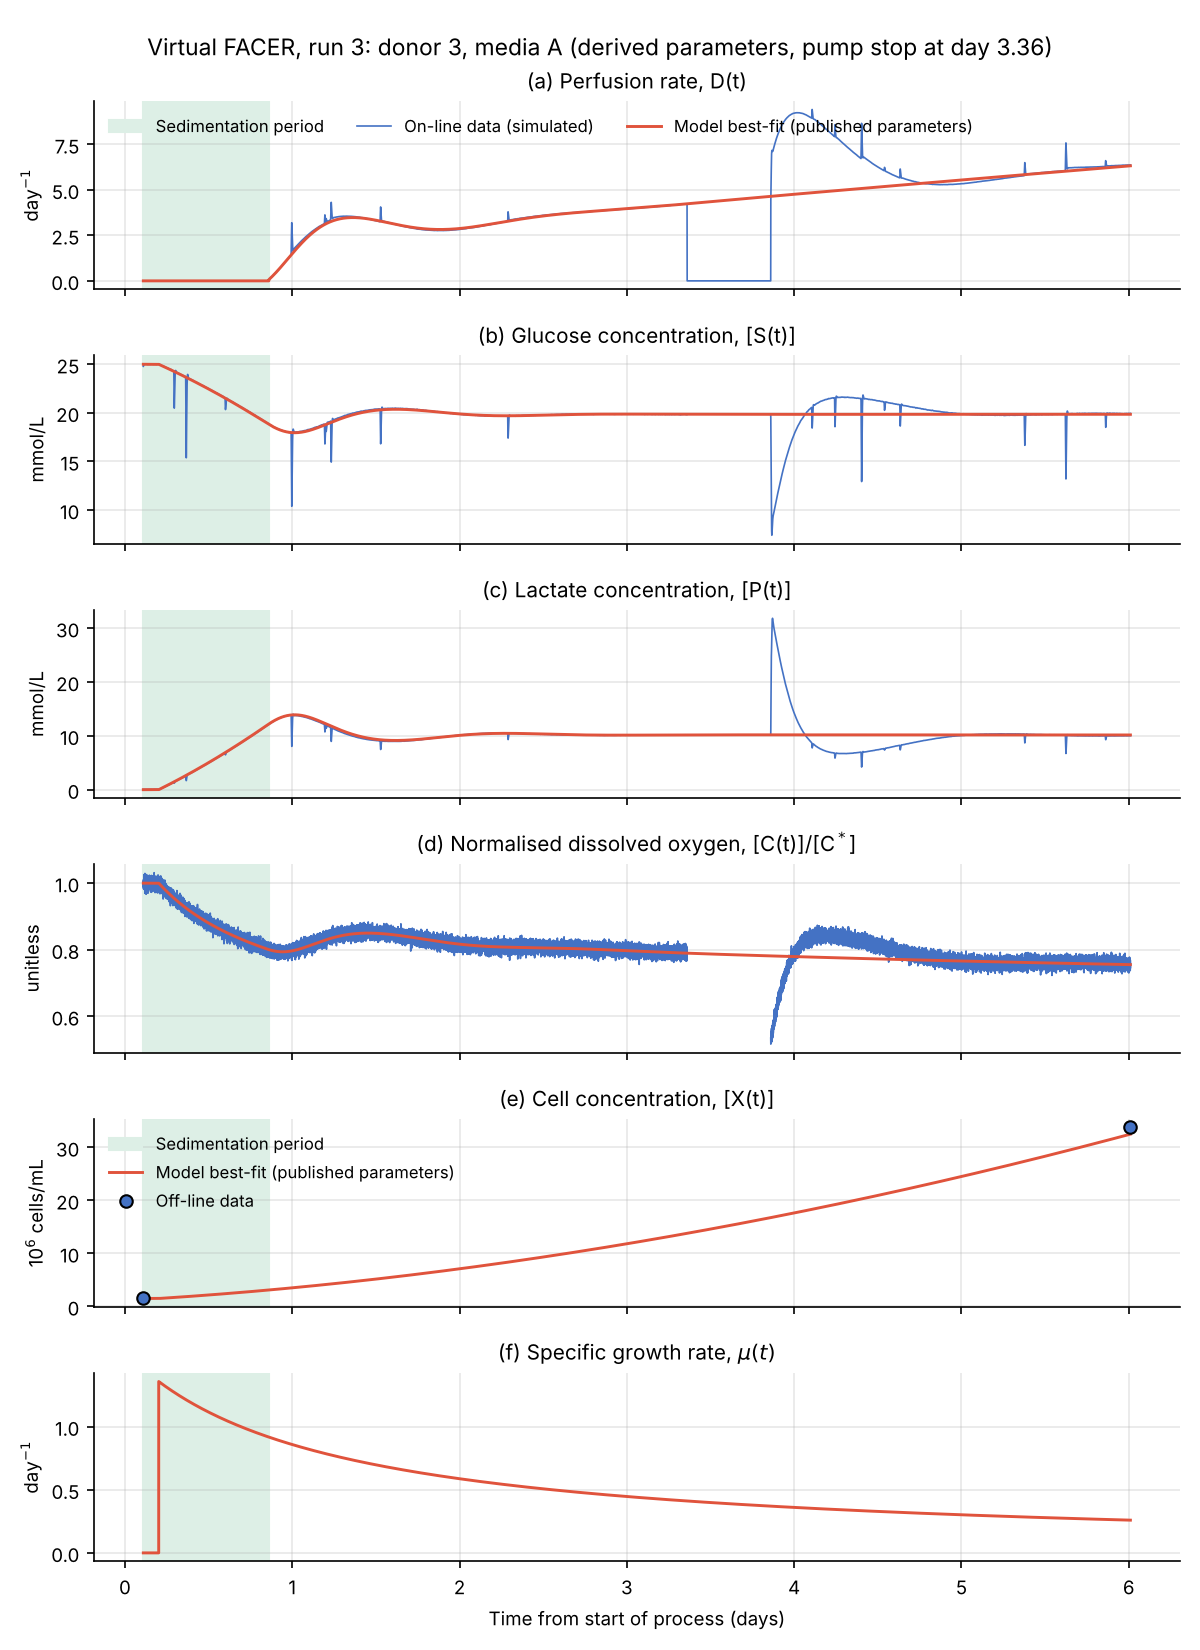
\includegraphics[width=0.8\textwidth]{figures/run3.png}
\caption{Key data from virtual run~3 with the mechanical issue 2.5~days following the start of
perfusion, during which no online data were recorded.}
\label{fig:run3}
\end{figure}

\subsection{Digital shadow training}
Table~\ref{tab:train} shows the best-fit parameters for the five training runs. The yields are
recovered to within 5\% ($Y_{xs}$) and 7\% ($Y_{px}$) of the parameters used to generate the data, and
$\nu$ and the lag period are recovered closely. The deviations are attributable to the 5\% off-line
counting error, which propagates into $Y_{xs}$ through $\mumax$, and to bubble artefacts, which bias the
filtered lactate signal downwards and hence $Y_{px}$. The reduced chi-squared values are below unity
because the residuals are dominated by the filtered (and therefore smoothed) sensor noise.

\begin{table}[h]
\centering\small
\caption{Best-fit parameters with 95\% confidence intervals for the five virtual training runs, and
the values used to generate the data in square brackets (Table~2 of \cite{egan2025}).}
\label{tab:train}
\resizebox{\textwidth}{!}{%
\begin{tabular}{@{}l l l l l r@{}}
\toprule
Run & $Y_{xs}$ & $Y_{px}$ & $\tlag-t_I$ & $\nu$ & $\chi^2_n$ \\
\midrule
1 & 0.241 (0.236, 0.246) [0.231] & 7.51 (7.36, 7.66) [7.93] & 0.162 (0.047, 0.278) [0.160] & $-0.895$ ($-0.905$, $-0.886$) [$-0.922$] & 0.11 \\
2 & 0.282 (0.281, 0.282) [0.275] & 6.02 (6.00, 6.03) [6.25] & 0.171 (0.145, 0.197) [0.172] & $-0.473$ ($-0.478$, $-0.468$) [$-0.477$] & 0.11 \\
4 & 0.282 (0.280, 0.283) [0.272] & 8.65 (8.61, 8.69) [9.09] & 0.124 (0.079, 0.169) [0.128] & $-0.527$ ($-0.536$, $-0.518$) [$-0.524$] & 0.08 \\
5 & 0.215 (0.214, 0.216) [0.207] & 6.52 (6.49, 6.56) [6.83] & 0.000 (0.000, 0.072) [0.000] & $-0.011$ ($-0.026$, $0.000$) [$-0.000$] & 0.06 \\
6 & 0.321 (0.318, 0.324) [0.311] & 7.63 (7.55, 7.70) [7.99] & 0.000 (0.000, 0.072) [0.000] & $-0.762$ ($-0.772$, $-0.752$) [$-0.761$] & 0.09 \\
\bottomrule
\end{tabular}}
\end{table}

\subsection{Digital shadow testing}
Figure~\ref{fig:rt} shows the relative errors of the predicted final cell concentration with varying
quantities of online data, and the cell concentration predictions based on 2.5~days of online data
(cf.\ Figures~5 and~6 of \cite{egan2025}); Table~\ref{tab:rt} lists the values. With 1.5~days of
online data, five of the six runs are predicted to within a 30\% relative error. With 2.5~days (or
more) of online data, the final cell concentration is predicted to within a 30\% relative error for
all runs, with a mean relative error of 8\% (Egan et al.: 13\%, standard deviation $\approx$ 6\%).

\begin{figure}[h]
\centering
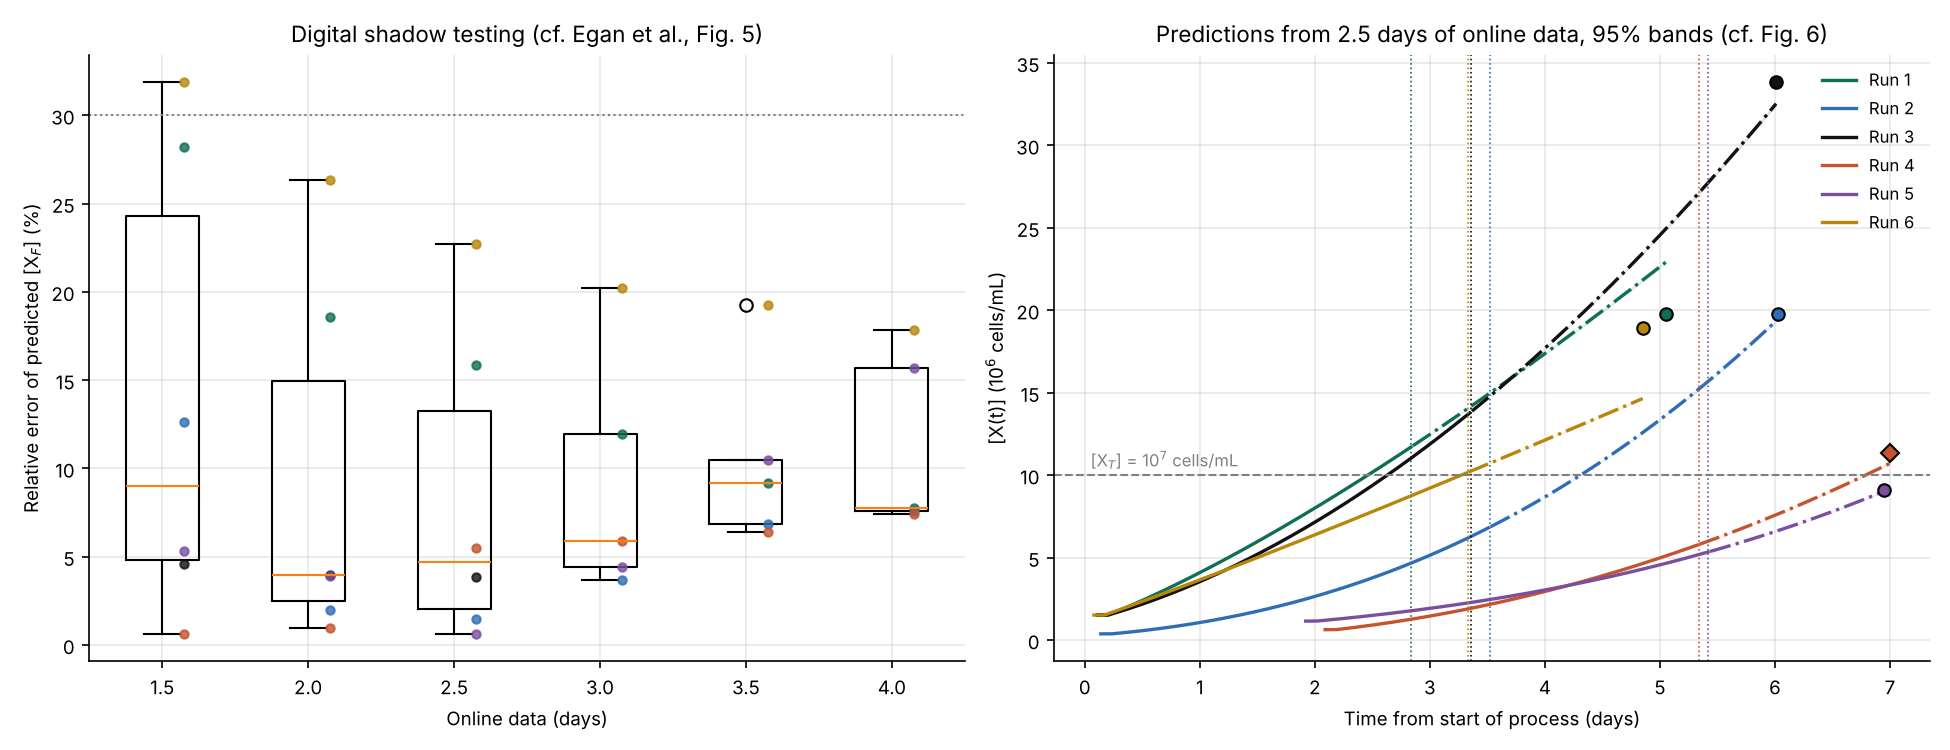
\includegraphics[width=\textwidth]{figures/realtime_test.png}
\caption{Left: relative errors of predicted final cell concentration with varying quantities of online
data. Right: cell concentration predictions based on 2.5~days of online data and the off-line initial
cell concentration; solid lines are predictions up to the time of fitting, dash-dotted lines future
predictions, dotted vertical lines the time of fitting and symbols the off-line final cell
concentrations (diamond: patient~1).}
\label{fig:rt}
\end{figure}

\begin{table}[h]
\centering\small
\caption{Relative error (\%) of the predicted final cell concentration.}
\label{tab:rt}
\begin{tabular}{@{}l r r r r r r r@{}}
\toprule
Online data (days) & Run 1 & Run 2 & Run 3 & Run 4 & Run 5 & Run 6 & Mean absolute \\
\midrule
1.5 & 28.2 & 12.7 & $-4.6$ & 0.6 & $-5.3$ & $-31.9$ & 13.9 \\
2.0 & 18.6 & 2.0 & $-4.0$ & $-0.9$ & $-3.9$ & $-26.3$ & 9.3 \\
2.5 & 15.8 & $-1.5$ & $-3.9$ & $-5.5$ & $-0.6$ & $-22.7$ & 8.3 \\
3.0 & 12.0 & $-3.7$ & -- & $-5.9$ & 4.4 & $-20.2$ & 9.2 \\
3.5 & 9.2 & $-6.9$ & -- & $-6.4$ & 10.5 & $-19.2$ & 10.4 \\
4.0 & 7.7 & $-7.6$ & -- & $-7.4$ & 15.7 & $-17.8$ & 11.3 \\
\bottomrule
\end{tabular}
\end{table}

The confidence bands are too narrow, in that the final cell concentration is frequently not within the
band. Runs~1 and~6 are consistently over- and under-predicted, respectively, irrespective of the
quantity of online data. Their yields of cells from glucose (0.231 and 0.311~cells/pmol) differ from
the fixed mean value (0.259~cells/pmol) by $-11\%$ and $+20\%$; since the digital shadow infers the
growth of cells from their glucose consumption via $Y_{xs}$, this deviation propagates directly into
the predicted cell concentration and is not captured by the confidence bands of
equation~\eqref{eq:band}.

% =====================================================================
\section{Discussion}

The virtual bioreactor reproduces the published parameter values, the qualitative features of the
published online data (the transient response of the PI(D) controller, the stabilisation of the
glucose concentration at its set-point, the steady state of the lactate concentration, and the bubble
artefacts that survive the filter) and the mechanical issue of run~3. Within this environment, the
re-implemented digital shadow reproduces the main findings of Egan et al.: the training parameters are
recovered, and with at least 2.5~days of online data the final cell concentration is predicted with a
relative error of less than 30\%.

As in the original study, the confidence bands should be interpreted as minimum confidence bands,
because other sources of uncertainty are not captured: the uncertainty in $Y_{xs}$ and $\tlag$, the
uncertainty in the online and off-line measurements, and the uncertainty in the model structure.
Egan et al.\ proposed fitting a bivariate distribution to the parameter estimates of $Y_{xs}$ and
$\tlag$ from many runs, repeatedly sampling from that distribution and using the sampled values when
fitting to the online data in real time, to obtain a distribution of predicted cell concentrations.
This is an ensemble approach, and an ensemble Kalman filter formulation of the digital shadow, in
which $Y_{xs}$ and $\tlag$ are treated as uncertain augmented states, is a natural extension.

The strongest assumption of the model is that the media and cells are homogeneously mixed, although
the cells are sedimented on the membrane and the influent and effluent are situated higher up. The
model further assumes that all cells are homogeneous; T cells comprise CD4$^+$ and CD8$^+$ subsets
with different expansion profiles, which an extension to a segregated model could address. In the
virtual bioreactor, these assumptions hold by construction, so the reported errors reflect parameter
and measurement uncertainty only, and not model structure uncertainty.

Other limitations are specific to this re-implementation: the online data are synthetic, since the
original datasets are proprietary; the noise levels and bubble statistics are assumed values; and the
parameters of run~3 are assigned rather than estimated.

% =====================================================================
\section{Conclusion}

A digital shadow of CAR T cell expansion in a PID controlled perfusion bioreactor has been
re-implemented, together with a virtual bioreactor that generates online and off-line data from the
published parameters of six bioreactor runs of the Aglaris FACER. The digital shadow provides nowcasts
and short-term forecasts of the cell concentration, and hence of the time at which a threshold cell
concentration is reached, using only the hard sensors already used to monitor and control the process.
The virtual bioreactor provides a test environment for further work: exposing the bioreactor via
industrial communication protocols, an ensemble-based digital shadow that captures the uncertainty in
$Y_{xs}$ and $\tlag$, decision support for the harvest time with the human operator in the loop, and
tuning of the PID parameters via the digital shadow, which Egan et al.\ identify as a means to improve
the stability of the glucose concentration around its set-point.

% =====================================================================
\section*{Nomenclature}
\begin{center}\small
\begin{longtable}{@{}p{0.27\textwidth} p{0.45\textwidth} p{0.22\textwidth}@{}}
\toprule
Symbol & Description & Units \\
\midrule
$t$ & time from the start of the process & days \\
$t_I$, $\tsed$, $t_F$ & initial (seeding), final sedimentation and final perfusion times & days \\
$\tlag$ & time at which cell growth starts; $\tlag-t_I$ is the lag period & days \\
$t_T$ & time at which $\cX$ reaches $[X_T]$ & days \\
$\cX$, $[X_I]$, $[X_F]$, $[X_T]$ & cell concentration; initial, final and threshold values & \num{e6} cells/mL \\
$\cS$, $[S_I]$, $\Ssp$ & glucose concentration; in fresh media; set-point & mmol/L \\
$\cP$, $[P_{ss}]$ & lactate concentration; steady state & mmol/L \\
$C'(t) = [C(t)]/[C^*]$ & normalised dissolved oxygen & unitless \\
$D(t)$, $D_{\min}$ & perfusion rate; minimum perfusion rate & day$^{-1}$ \\
$Q(t)$, $V$ & volumetric flow rate; bioreactor volume & mL/day; mL \\
$\mu(t)$, $\mumax$ & specific growth rate; maximum specific growth rate & day$^{-1}$ \\
$\nu$ & decrease of specific growth rate & unitless \\
$[K]$ & carrying capacity & \num{e6} cells/mL \\
$Y_{xs}$ & yield of cells from glucose & cells/pmol \\
$Y_{px}$ & yield of lactate from cells & pmol/cell \\
$Y_{ps}$ & yield of lactate from glucose & unitless \\
$\kla$, $Y'_{xc}$ & volumetric mass transfer coefficient; scaled yield of cells from DO & day$^{-1}$; \num{e6} cells/mL \\
$K_p$, $K_i$, $K_d$ & proportional, integral and derivative gains & L/(mmol\,day); L/(mmol\,day$^2$); L/mmol \\
$H$ & Heaviside step function & -- \\
$\chi^2_n$ & reduced chi-squared & unitless \\
\bottomrule
\end{longtable}
\end{center}

% =====================================================================
\section*{Appendix: implementation and verification}
\begin{center}\small
\begin{tabularx}{\textwidth}{@{}l X@{}}
\toprule
\code{process/growth.py} & equations~\eqref{eq:X}--\eqref{eq:closed}, \eqref{eq:Pss}; sensitivities S67--S70 \\
\code{process/parameters.py} & Table~\ref{tab:runs}; mean training values \\
\code{process/facer.py} & equations~\eqref{eq:S22}--\eqref{eq:S24} and~\eqref{eq:DO}; the model fitted by the digital shadow \\
\code{control/perfusion.py} & PID controller, equation~\eqref{eq:pid} \\
\code{control/pid.py} & generic PI controller with anti-windup (control refresher notes) \\
\code{sensors/online.py} & enzymatic sensors, bubble artefacts, Butterworth filter, DO, off-line counts \\
\code{sim/runner.py} & virtual bioreactor, mechanical issue, data export \\
\code{shadow/fit.py} & digital shadow training and testing, confidence bands, $t_T$ \\
\code{scripts/simulate\_run.py}, \code{scripts/realtime\_test.py} & Figures~\ref{fig:run1}, \ref{fig:run3} and~\ref{fig:rt}; Table~\ref{tab:rt} \\
\bottomrule
\end{tabularx}
\end{center}
The test suite (\code{pytest}, 31 tests) verifies the special cases of the growth model,
$\mu(t)=\dd\ln\cX/\dd t$, the agreement of $\mumax$ and $t_T-t_I$ with Table~2, the mutual consistency of
equation~\eqref{eq:closed}, the analytical sensitivities against finite differences, the final cell
concentrations, set-point tracking and lactate steady state of every run, the absence of perfusion
during the sedimentation period, the filter and bubble models, the mechanical issue of run~3, the
recovery of the training parameters, the 30\% bound of digital shadow testing with 2.5~days of online
data, and the narrowing of the confidence bands with increasing online data.

\begin{thebibliography}{9}
\bibitem{egan2025} Egan JR, Mar\'i-Buy\'e N, Ben\'itez-Cano EV, Costa M, Wanika L, Chappell MJ,
  Schultz U, Ochs J, Effenberger M, Horna D, Rafiq Q, Goldrick S. A digital shadow of CAR T cell
  expansion in a perfusion bioreactor: informing optimal harvest times for autologous cell therapy.
  \emph{Biotechnol Prog.} 2025;41(6):e70045. \href{https://doi.org/10.1002/btpr.70045}{doi:10.1002/btpr.70045}
\bibitem{richards1959} Richards FJ. A flexible growth function for empirical use. \emph{J Exp Bot.}
  1959;10(2):290--301. doi:10.1093/jxb/10.2.290
\end{thebibliography}

\end{document}
